%\section{Einleitung}
\subsection{Factory}
\begin{frame}
  \frametitle{Factory}
  \framesubtitle{Idee}
  \begin{itemize}
    \item Objekterstellung mittels separater Klasse
    \item Kann Client-Code von den konkreten Implementierungsdetails entkoppeln
    \item Verschiedene Implementierungen können unterstützt werden
    \item Kann Komplexität kapseln
    \item Ressourcen können zentral erstellt und verwaltet werden
    \item Kann Load Balancing und Failover-Mechanismen implementieren
  \end{itemize}
\end{frame}


\begin{frame}
  \frametitle{Factory}
  \framesubtitle{Pattern}
  \begin{figure}[!ht]
    \centering
    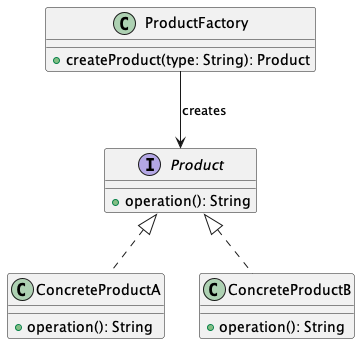
\includegraphics[width=0.45\textwidth]{fig/uml/factory-class.png}
    \caption{Factory Pattern}
    \label{fig:factory-class}
  \end{figure}
\end{frame}

\begin{frame}
  \frametitle{Factory}
  \framesubtitle{Sequenz}
   \begin{figure}[!ht]
    \centering
    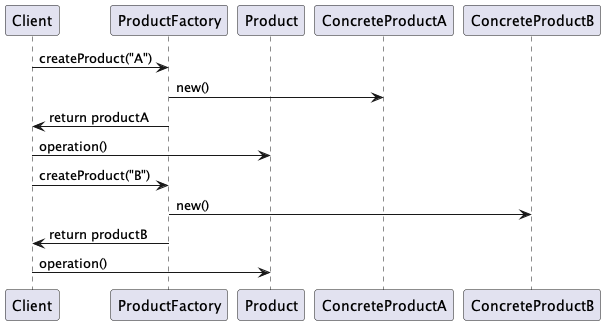
\includegraphics[width=0.85\textwidth]{fig/uml/factory-seq.png}
    \caption{Factory Pattern Sequenz}
    \label{fig:factory-seq}
  \end{figure}
\end{frame}

\begin{frame}
  \frametitle{Factory}
  \framesubtitle{Diskussion Eignung}
  \begin{itemize}
    \item Code sauberer und wartbarer
    \item Skalierbarkeit und Fehlertoleranz verbessert
    \item Viele Probleme bleiben: Kommunikationslatenz, Synchronisation, SPOF, Komplexität, Testbarkeit, Overhead
    \item Meist besser als Singleton
  \end{itemize}
\end{frame}